\documentclass[compress, 9pt]{beamer}

%\usepackage{beamerthemesplit}
\graphicspath{{Figures/}}
%\usetheme[height=1cm]{Rochester}
%\usetheme[height=1cm]{Singapore}
%\usetheme{Boadilla}
%\usetheme{boxes}
\usetheme[height=1cm]{Boadilla}
%\useoutertheme[footline=authortitle,subsection=false,height=1cm]{miniframes}
%\useoutertheme[subsection=false,height=1cm]{smoothbars}
\usepackage{epic}
%\usepackage{natbib}
%\usepackage[notocbib]{apalike}
\usepackage{color}
\beamertemplatenavigationsymbolsempty
\usepackage{graphicx}
\usepackage{color}
\usepackage[mathscr]{eucal}
\usepackage{epsfig}
\usepackage[all]{xy}
\usepackage{url}
\usepackage{setspace}

\DeclareMathOperator{\E}{E}
\DeclareMathOperator{\I}{I}
\DeclareMathOperator{\Var}{Var}
\DeclareMathOperator{\Cov}{Cov}
\DeclareMathOperator{\logit}{logit}
\DeclareMathOperator{\dom}{dom}
\DeclareMathOperator{\cl}{cl}
\DeclareMathOperator{\bd}{bd}
\DeclareMathOperator{\rbd}{rbd}
\DeclareMathOperator{\intr}{int}
\DeclareMathOperator{\rint}{rint}
\DeclareMathOperator{\con}{con}
\DeclareMathOperator{\pos}{pos}
\DeclareMathOperator{\aff}{aff}
\DeclareMathOperator{\epi}{epi}
\DeclareMathOperator{\lev}{lev}
\DeclareMathOperator{\spanl}{span}

\def\RR{{\mathbb R}}
\def\ZZ{{\mathbb Z}}
\def\DD{{\mathcal D}}
\def\XX{{\mathcal X}}
\def\YY{{\mathcal Y}}
\def\TT{{\mathcal T}}
\def\NN{{\mathcal N}}
\newcommand{\deriv}[2]{\frac{d #1}{d #2}}
\newcommand{\dderiv}[2]{\frac{d^2 #1}{d #2^2}}
\newcommand{\pderiv}[2]{\frac{\partial #1}{\partial #2}}
\newcommand{\ppderiv}[2]{\frac{\partial^2 #1}{\partial #2^2}}
\newcommand{\ppmderiv}[3]{\frac{\partial^2 #1}{\partial #2 \partial #3}}
\newcommand{\fatdot}{\,\cdot\,}
\newcommand{\inner}[1]{\langle #1 \rangle}
\newcommand{\set}[1]{\{\, #1 \,\}}
\newcommand{\abs}[1]{\lvert #1 \rvert}
\newcommand{\norm}[1]{\lVert #1 \rVert}
\newcommand{\etaMLE}{\hat{\eta}_{\textrm{MLE}}}
\newcommand{\betaMLE}{\hat{\beta}_{\textrm{MLE}}}
\newcommand{\thetaLCM}{\hat{\theta}_{\textrm{LCM}}}
\newcommand{\etaLCM}{\hat{\eta}_{\textrm{LCM}}}
\newcommand{\yobs}{y_{\text{obs}}}
\newcommand{\Gammalim}{\Gamma_{\textrm{lim}}}
\newcommand{\CLCM}{C_{\textrm{LCM}}}

\setbeamercovered{transparent}

\title{Parameter Estimation in Social Network Models}
\author{
  Saisuke Okabayashi %\\
%  Charles J. Geyer
  }

\institute{Department of Statistics \\ University of Minnesota}

\date{April 5, 2011}


\begin{document}
%\usefoottemplate{\vbox{\tinycolouredline{structure!75}{\color{white}\textbf{\insertauthor\hfill}}\tinycolouredline{structure}{\color{white}\textbf{\inserttitle}\hfill}}}

\frame{\titlepage}
\section{Background}
\frame{
	\frametitle{My research is about}
\begin{itemize}
\item optimization
\item curvature condition
\item linear programming
\item relative boundaries of convex hulls
\item directions of recession
\end{itemize}

But that's not how it began!
}


\frame
{
  \frametitle{It began with some monks ...}
\begin{figure}
\begin{center} 
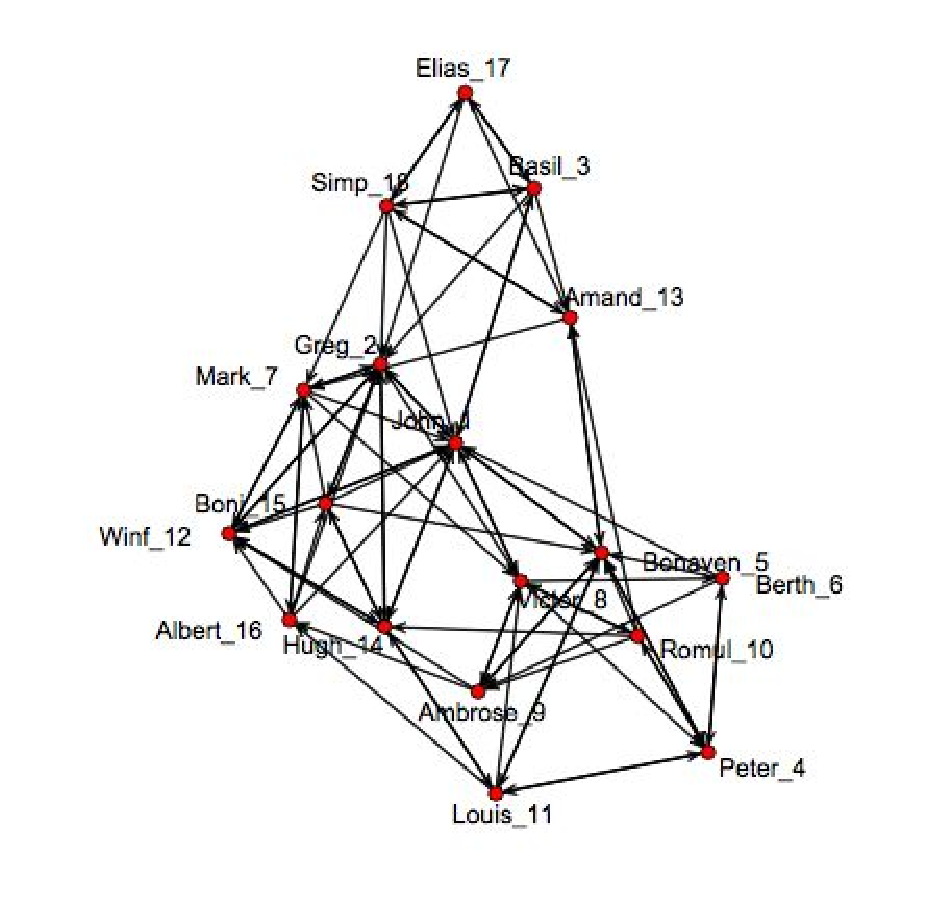
\includegraphics[height=3in]{samplike}
\caption{Sampson's (1969) monastery affinity network.} 
\end{center} 
\label{fmh} 
\end{figure}
}
\frame
{
  \frametitle{and... }
\begin{figure}
\begin{center} 
\includegraphics[height=3in]{fmh-gradesex2}
\caption{Adolescent Health friendship network.} 
\end{center} 
\label{fmh} 
\end{figure}
}
\frame
{
  \frametitle{and... }

\begin{figure}
\begin{center} 
\includegraphics[height=3in]{florentine}
\caption{Florentine marriage network.} 
\end{center} 
\label{fmh} 
\end{figure}
}
\frame
{
  \frametitle{and...}

\begin{figure}
\begin{center} 
\scalebox{.4}{\includegraphics{ecoli}}
\caption{E. coli network.} 
\end{center} 
\label{fmh} 
\end{figure}
}

\frame
{
\frametitle{Why networks?}
Networks are a conduit for \emph{flow}.  

Flow can be friendship, diseases, data, airplanes, commodities, ideas, advice, association.

Network models can help explain the mechanism of this flow.
}

%%%%%%%%%%%%%%%%%%%%%%%%%%%%%%%%%%%%%%%%%%%%%%%%%%%%%%%%%%%%%
\section{Modeling}
\frame
{
\frametitle{A network as a matrix}
Formally, a social network is a collection of actors and the relations, or ties, between each 
pair of actors.  

We can represent a network with $n$ actors as an $n \times n$ matrix $Y$, where each entry
\begin{align*}
	Y_{ij} =
	\begin{cases} 	1 \quad \text{if a relation exists from actor $i$ to actor $j$}\\
					0 \quad \text{otherwise}
	\end{cases}
\end{align*}

The Florentine marriage network, in matrix form:
{\tiny
\begin{table}[htdp]
\begin{center}\begin{tabular}{|c|c|c|c|c|c|c|c|c|c|c|c|c|c|c|c|}
\hline 
0 & 0 & 0 &     0 &     0 &     0 &     0 &     0 &     1&      0 &      0 &      0 &      0 & 0 &      0 &      0 \\ \hline
0 & 0 &     0 &     0 &     0 &     1&     1&     0 &     1&      0 &      0 &      0 & 0 &      0 &      0 &      0 \\  \hline
0 & 0 &     0 &     0 &     1&     0 &     0 &     0 &     1&      0 &      0 &      0 & 0 &      0 &      0 &      0 \\  \hline
0 & 0 &     0 &     0 &     0 &     0 &     1&     0 &     0 &      0 &      1&      0 & 0 &      0 &      1&      0 \\  \hline
0 & 0 &     1&     0 &     0 &     0 &     0 &     0 &     0 &      0 &      1&      0 & 0 &      0 &      1&      0 \\  \hline
0 & 1&     0 &     0 &     0 &     0 &     0 &     0 &     0 &      0 &      0 &      0 & 0 &      0 &      0 &      0 \\   \hline
0 & 1&     0 &     1&     0 &     0 &     0 &     1&     0 &      0 &      0 &      0 &  0 &      0 &      0 &      1 \\  \hline
0 & 0 &     0 &     0 &     0 &     0 &     1&     0 &     0 &      0 &      0 &      0 & 0 &      0 &      0 &      0 \\  \hline
1& 1&     1&     0 &     0 &     0 &     0 &     0 &     0 &      0 &      0 &      0 &  1&      1&      0 &      1\\  \hline
0 & 0 &     0 &     0 &     0 &     0 &     0 &     0 &     0 &      0 &      0 &      0 & 0 &      1&      0 &      0 \\  \hline
0 &0 &     0 &     1&     1&     0 &     0 &     0 &     0 &      0 &      0 &      0 &    0 &      0 &      1&      0 \\  \hline
0 & 0 &     0 &     0 &     0 &     0 &     0 &     0 &     0 &      0 &      0 &      0 & 0 &      0 &      0 &      0 \\  \hline
0 & 0 &     0 &     0 &     0 &     0 &     0 &     0 &     1&      0 &      0 &      0 & 0 &      0 &      1&      1\\  \hline
0 & 0 &     0 &     0 &     0 &     0 &     0 &     0 &     1&      1&      0 &      0 & 0 &      0 &      0 &      0 \\   \hline
0 & 0 &     0 &     1&     1&     0 &     0 &     0 &     0 &      0 &      1&      0 &   1&      0 &      0 &      0 \\  \hline
0 & 0 &     0 &     0 &     0 &     0 &     1&     0 &     1&      0 &      0 &      0 & 1&      0 &      0 &      0\\ 
\hline \end{tabular} 
\end{center}
\label{defaulttable}
\end{table}
}
}

\frame
{
\frametitle{A network model}

Writing down an expression for a network model is easy.  

Exponential-family Random Graph Models (ERGM) have a log likelihood
\begin{align*}
	\ell( \eta) = \inner{\eta, g(\yobs)} - c(\eta)
\end{align*}
where
\begin{align*}
	c(\eta) = \log \sum_{y \in \YY} e^{\inner{\eta, g(y)}}.
\end{align*}

The natural statistic $g(y)$ is a vector of \emph{network statistics} of interest.  Some examples:
\begin{itemize}
	\item number of edges, $\sum$
	\item number of triangles
\end{itemize}


}

\frame
{
\frametitle{Choice of network statistics}

}
\frame
{
\frametitle{Number of graphs in $\YY$}

}

%%%%%%%%%%%%%%%%%%%%%%%%%%%%%%%%%%%%%%%%%%%%%%%%%%%%%%%%%%%%%
\section{Parameter estimation}
\frame
{
\frametitle{Calibrating}
What are the values for $\eta$ so that the model assigns the highest probability to the observed data?

Maximum likelihood estimators (MLE)!

But how do you find this value that maximizes the likelihood if you can't evaluate the likelihood?
}

\frame
{
\frametitle{Methods that are out there}
\begin{figure}
\begin{center} 
\scalebox{.4}{\includegraphics{mck.pdf}}
%\caption{Adolescent Health.} 
\end{center} 
\label{fmh} 
\end{figure}
}

%%%%%%%%%%%%%%%%%%%%%%%%%%%%%%%%%%%%%%%%%%%%%%%%%%%%%%%%%%%%%
\section{Long range algorithm}
\frame
{
\frametitle{Goal for our algorithm}
Prove that $\lVert \nabla \ell(\eta_k) \rVert \ \to 0$ as $k \to +\infty$.
}



\frame
{
\frametitle{Long range algorithm}
\begin{singlespace} 
{
\noindent Get an initial value, $\eta_0$.\\ 
Set $k=0$. \\
Calculate $\nabla \ell( \eta_k)$, the direction of steepest ascent. \\
Set $p_k = \nabla \ell( \eta_k)$. \\
\textbf{while}  $\lVert \nabla \ell( \eta_k) \rVert > \epsilon$ \\ 
\hspace{4mm} \indent	 
\textbf{Find} a step size $\alpha_k$ that satisfies the modified 
curvature condition
\begin{align*}
	 0 & \leq \nabla \ell( \eta_k + \alpha_k p_k)^T p_k \leq c \nabla \ell(\eta_k)^T 
p_k
\end{align*}
\indent for some $0 < c < 1$.  
%This condition requires $\alpha_k$ to fall within \\
%\indent the acceptable region in Figure \ref{F:alpha_region}. \\

$\eta_{k+1} = \eta_k + \alpha_k p_k$.\\
\indent Calculate $\nabla \ell( \eta_{k+1})$.\\
\indent \textbf{Find} the new search direction $p_{k+1}$, which must be an ascent 
direction. \\
\indent $k = k + 1$.  \\
\textbf{end while}\\
}
\end{singlespace}
}

\frame
{
  \frametitle{Curvature condition in detail}
\begin{align*}
	 0 & \leq \nabla \ell( \eta_k + \alpha_k p_k)^T p_k \leq c \nabla \ell(\eta_k)^T 
p_k
\end{align*}
\begin{figure}[h]
\centering
    \scalebox{.25}{\input{Figures/alphamax.pdf_t}}
	\caption{Acceptable region for step size $\alpha_k$ along a search direction $p_k$.}
\label{F:alpha_region}
\end{figure}
}

%%%%%%%%%%%%%%%%%%%%%%%%%%%%%%%%%%%%%%%%%%%%%%%%%%%%%%%%%%%%%
\section{Examples}
\frame
{
  \frametitle{Example: Monks}  
}

\frame
{
  \frametitle{Example: Teenage friendships}  
}

%%%%%%%%%%%%%%%%%%%%%%%%%%%%%%%%%%%%%%%%%%%%%%%%%%%%%%%%%%%%%
\section{non-Existent MLEs}
\frame
{
  \frametitle{MLE does not always exist}  


}

\frame
{
  \frametitle{Conditions}  
Convex support

Direction of recession
}

\frame
{
  \frametitle{Studies in ERGM}  
\begin{figure}[h]
\centering
\includegraphics[height=3in]{g9-hull}
\caption{Acceptable region for step size 
along a search direction according to modified curvature condition 
\eqref{E:curvature mod}.}
\label{F:g9-hull}
\end{figure}
Cheating!
}

%%%%%%%%%%%%%%%%%%%%%%%%%%%%%%%%%%%%%%%%%%%%%%%%%%%%%%%%%%%%%
\section{Algorithm extended}
\frame
{
\frametitle{Long range search to a place that doesn't exist}
How do we find it?

What is ``it"?
}

\frame
{
\frametitle{Case: MLE exists}  
\begin{figure}[h]
\centering
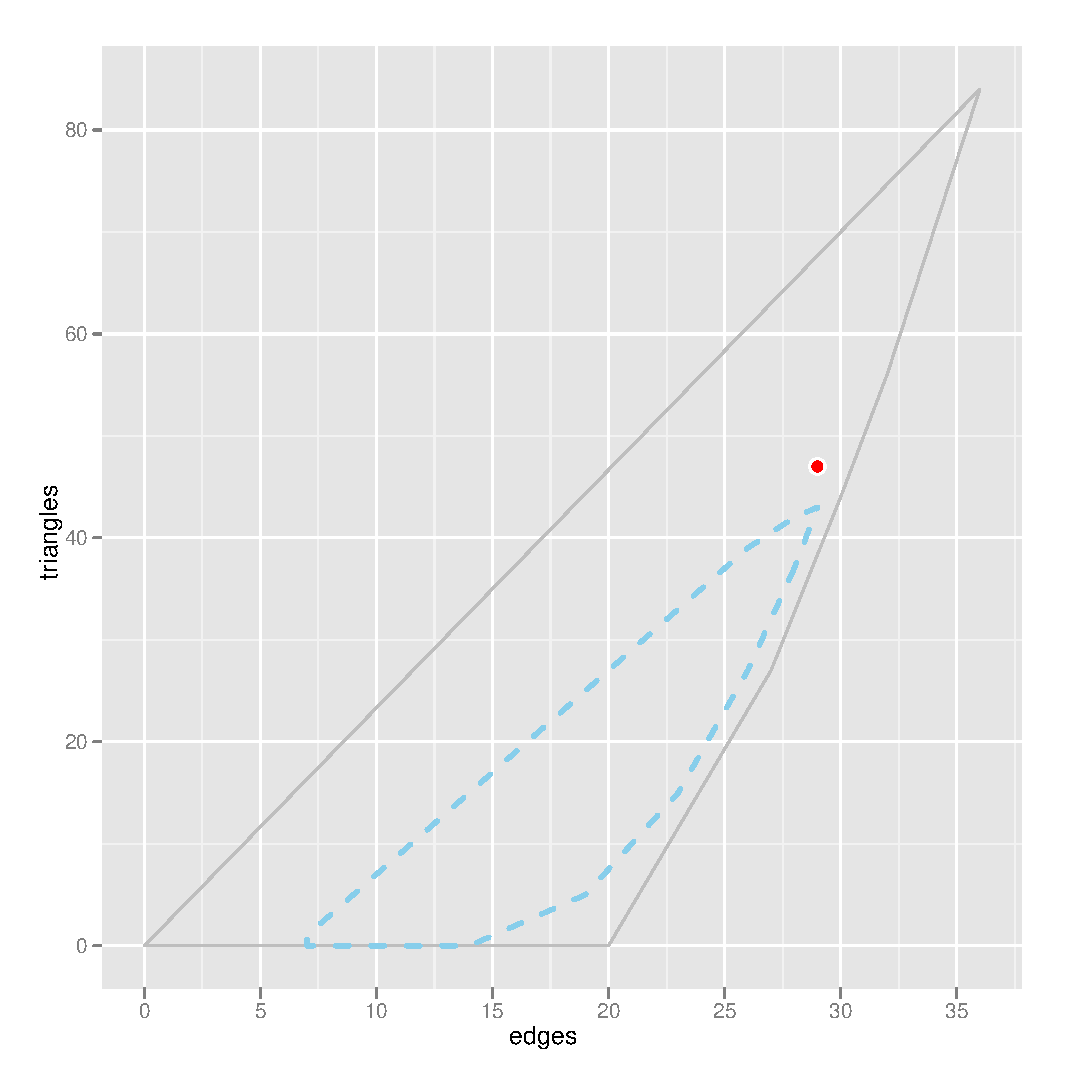
\includegraphics[height=2in]{MCsample-far}
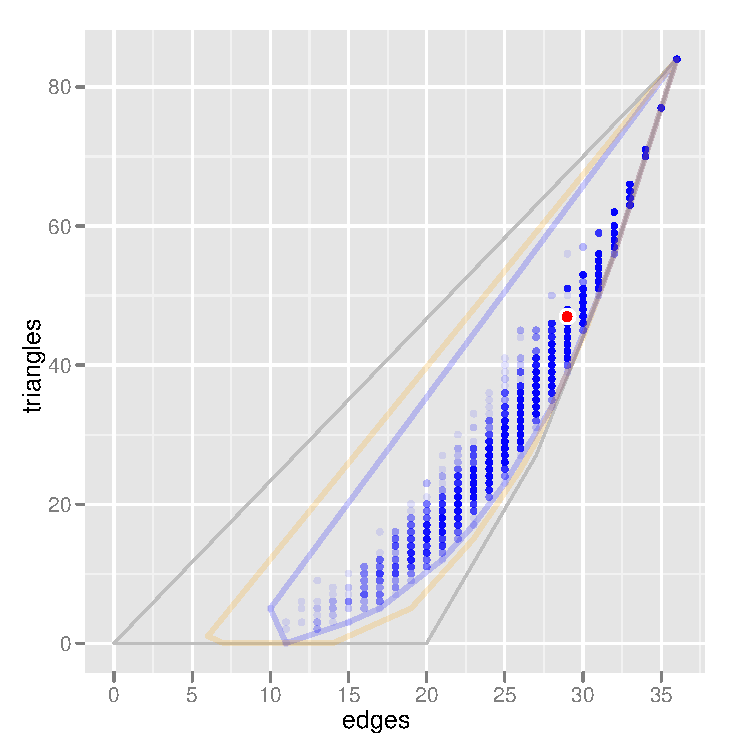
\includegraphics[height=2in]{MCsample-MLE}
\caption{MCMC samples when MLE exists.}
\label{F:MCsample-MLE exists}
\end{figure}
}


\frame
{
\frametitle{Case: MLE does not exists}  
\begin{figure}[h]
\centering
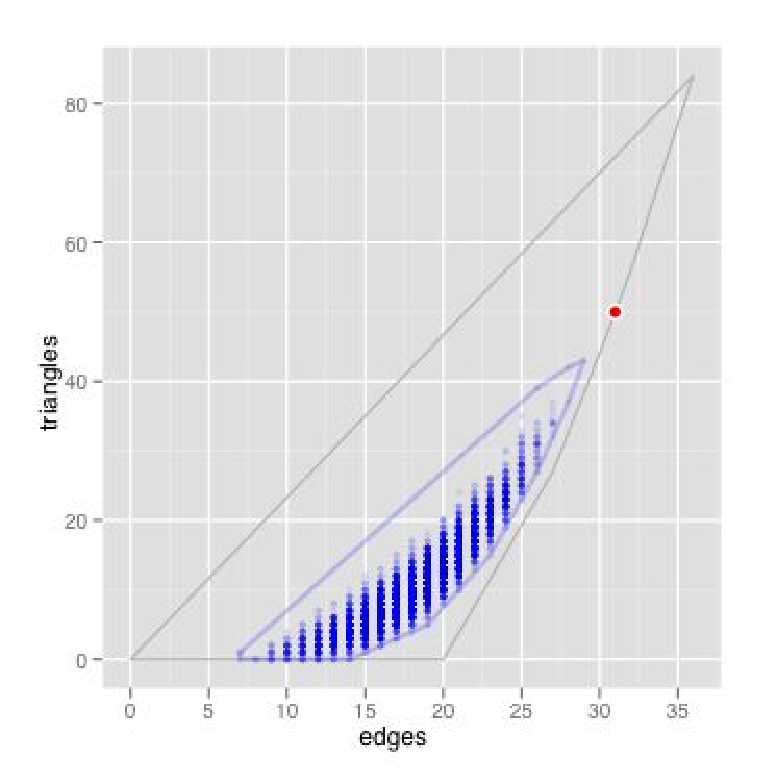
\includegraphics[height=2in]{MCsample-boundary}
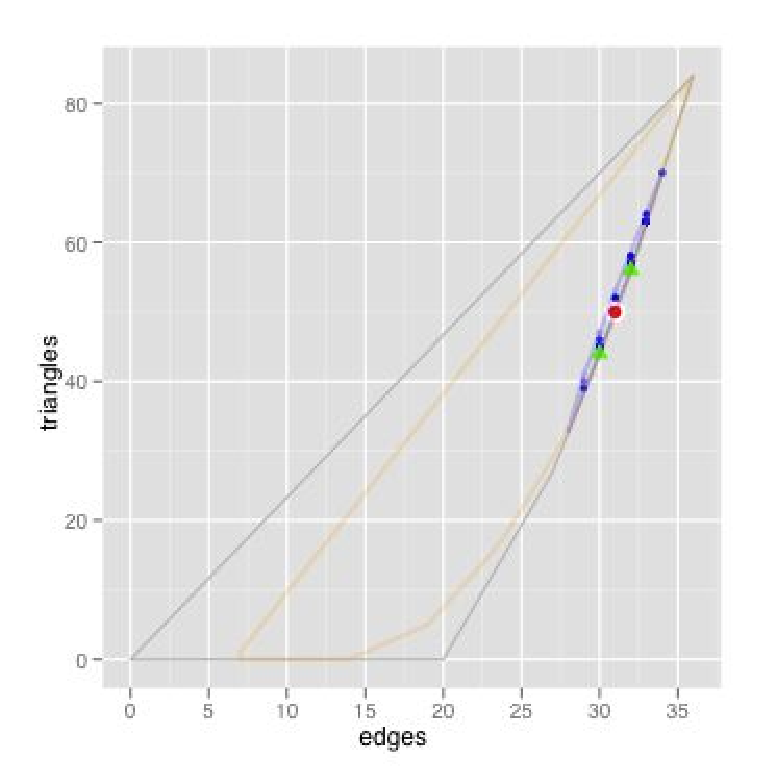
\includegraphics[height=2in]{MCsample-77face}
\caption{MCMC samples when MLE does not exist.}
\label{F:MCsample-MLE nonexistent}
\end{figure}
}


\frame
{
\frametitle{Case: MLE exists, but observed data close to boundary}  
\begin{figure}[h]
\centering
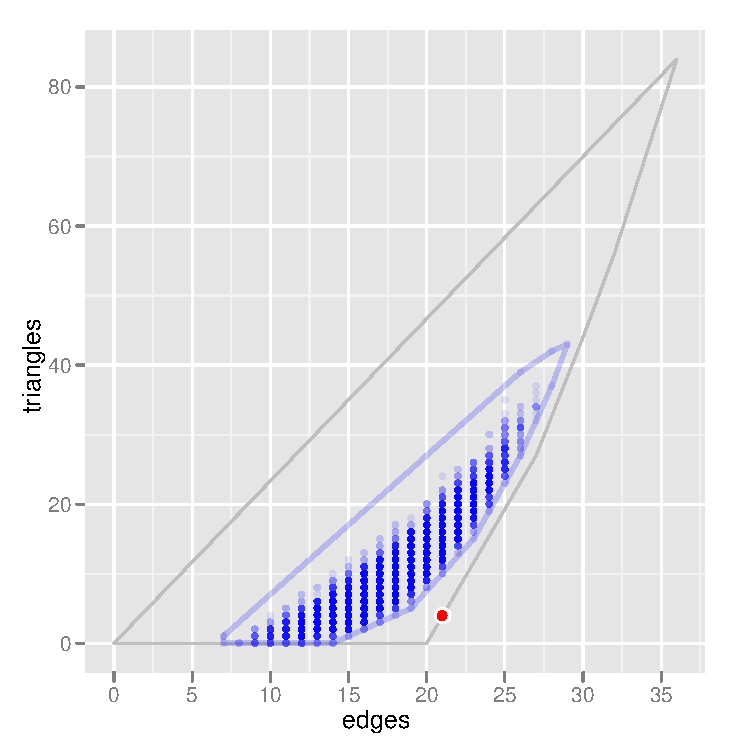
\includegraphics[height=2in]{MCsample-problem}
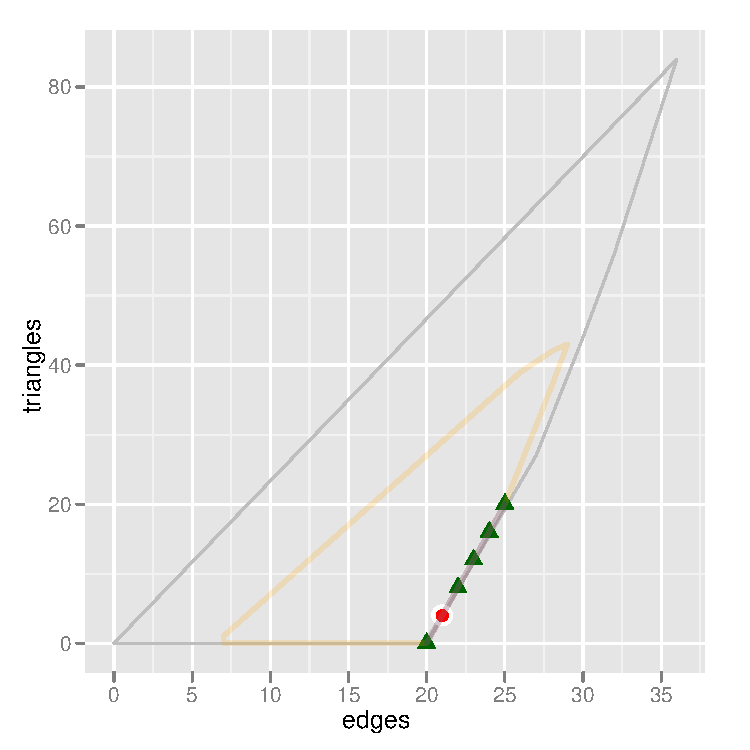
\includegraphics[height=2in]{MCsample-fakeface}
\caption{MCMC samples when MLE does not exist.}
\label{F:MCsample-MLE problem}
\end{figure}
}

\end{document}
